\section*{Unit}

\subsection*{Create new unit}

\begin{itemize}
  \item[] \textbf{Trigger:} User interaction with CMS window
  \item[] \textbf{Precondition:} Assert that user has logged in
  \item[] \textbf{Path:}
    \begin{enumerate}
      \item User clicks Admin on navigation bar
      \item User clicks on Units in the dropdown
      \item User clicks ``New Unit'' button
      \item User fills the unit information in the form
      \item User clicks ``Create Unit'' button
      \item ``Unit successfully created'' message is shown together with the data
    \end{enumerate}
  \item[] \textbf{Requirements:}
    \begin{enumerate}
      \item The new unit's data should be added to the database
      \item The new unit's information should be displayed in the homepage correctly
      \item The units' information should be listed in the creation order
    \end{enumerate}
  \item[] \textbf{Screenshots:} \\
    \includegraphics[scale=0.25]{./images/ss/unit/create/1.png}
    \includegraphics[scale=0.25]{./images/ss/unit/create/2.png}\\
    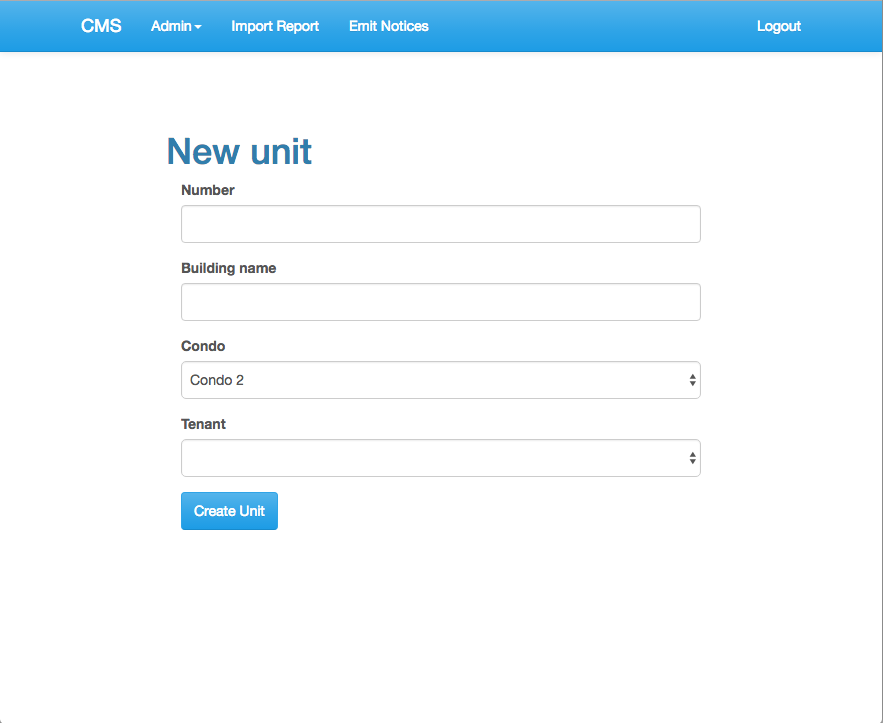
\includegraphics[scale=0.25]{./images/ss/unit/create/3.png}
    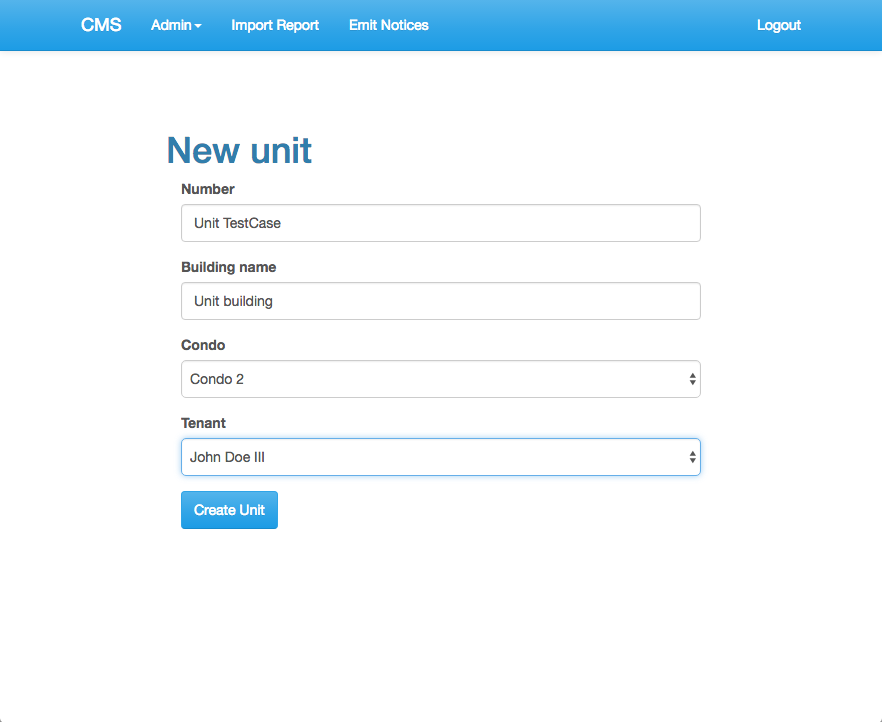
\includegraphics[scale=0.25]{./images/ss/unit/create/4.png}\\
    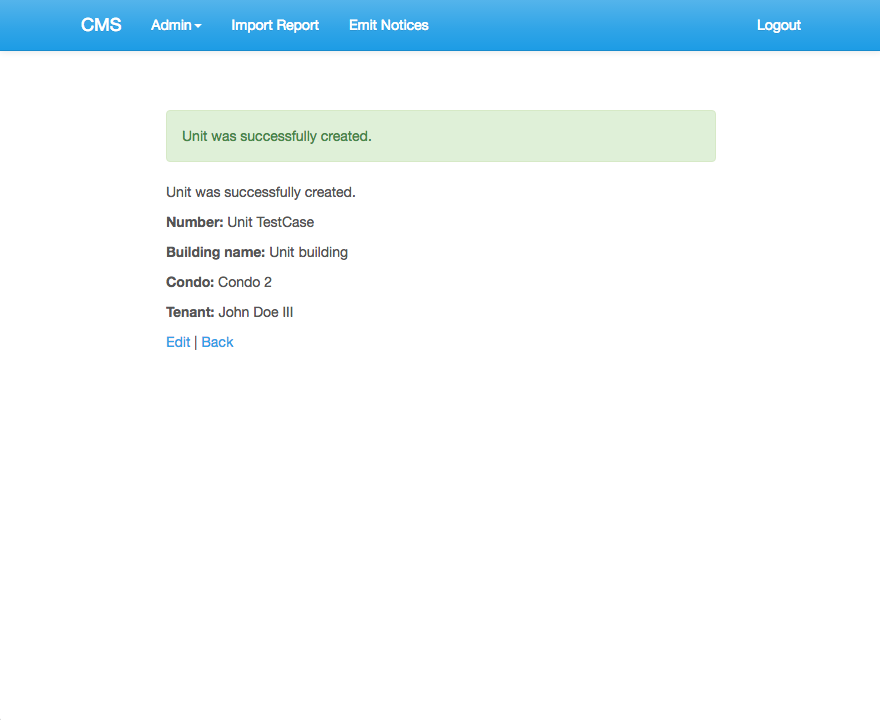
\includegraphics[scale=0.25]{./images/ss/unit/create/5.png}
\end{itemize}

\subsection*{Edit a unit}

\begin{itemize}
  \item[] \textbf{Trigger:} User interaction with CMS window
  \item[] \textbf{Precondition:} Assert that user is in the Unit page and the unit to edit is existed
  \item[] \textbf{Path:}
    \begin{enumerate}
      \item User clicks on Edit behind the information of the unit who will be edited
      \item User edit new information in the form
      \item User clicks ``Update Unit'' button
      \item ``Unit successfully updated'' massage is shown
    \end{enumerate}
  \item[] \textbf{Requirements:}
    \begin{enumerate}
      \item The updated unit’s new data should be updated to the database
      \item The updated unit’s new information should be displayed in the homepage correctly
      \item The units’ information should be listed in the modification order
    \end{enumerate}
  \item[] \textbf{Screenshots:}\\
    \includegraphics[scale=0.25]{./images/ss/unit/edit/1.png}
    \includegraphics[scale=0.25]{./images/ss/unit/edit/2.png}\\
    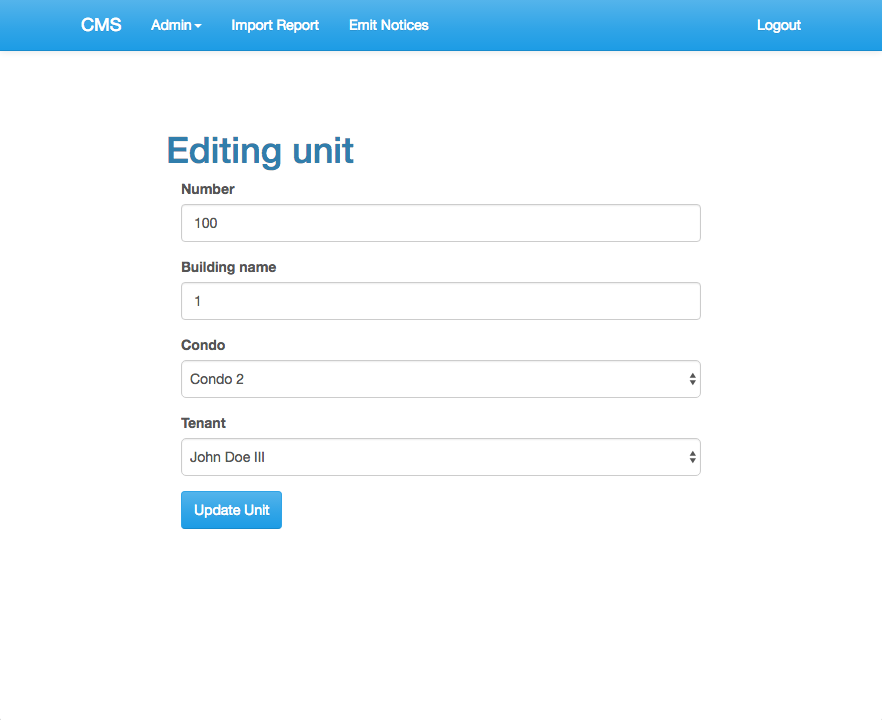
\includegraphics[scale=0.25]{./images/ss/unit/edit/3.png}
    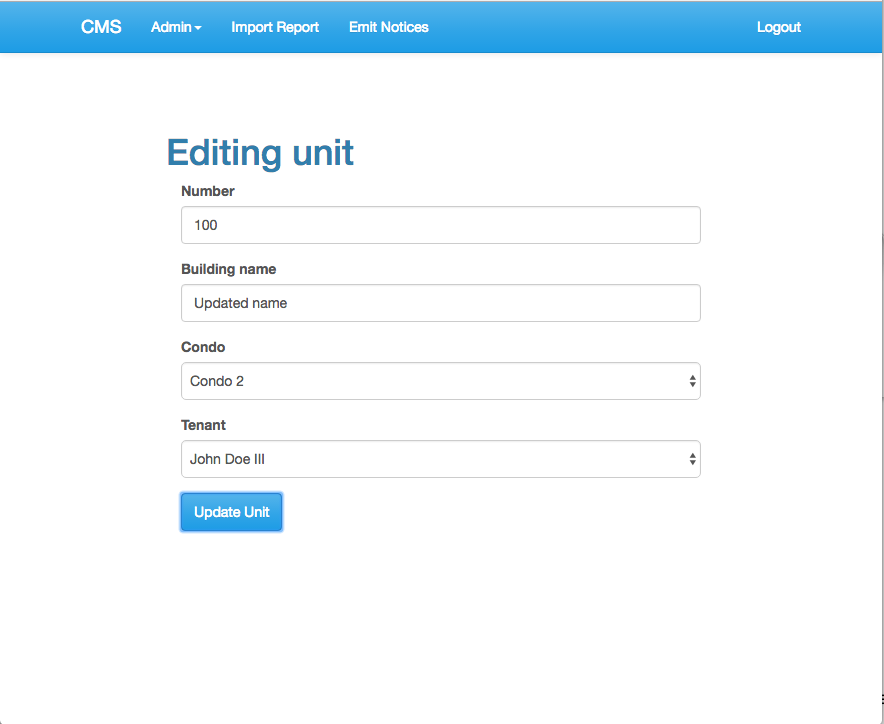
\includegraphics[scale=0.25]{./images/ss/unit/edit/4.png}\\
    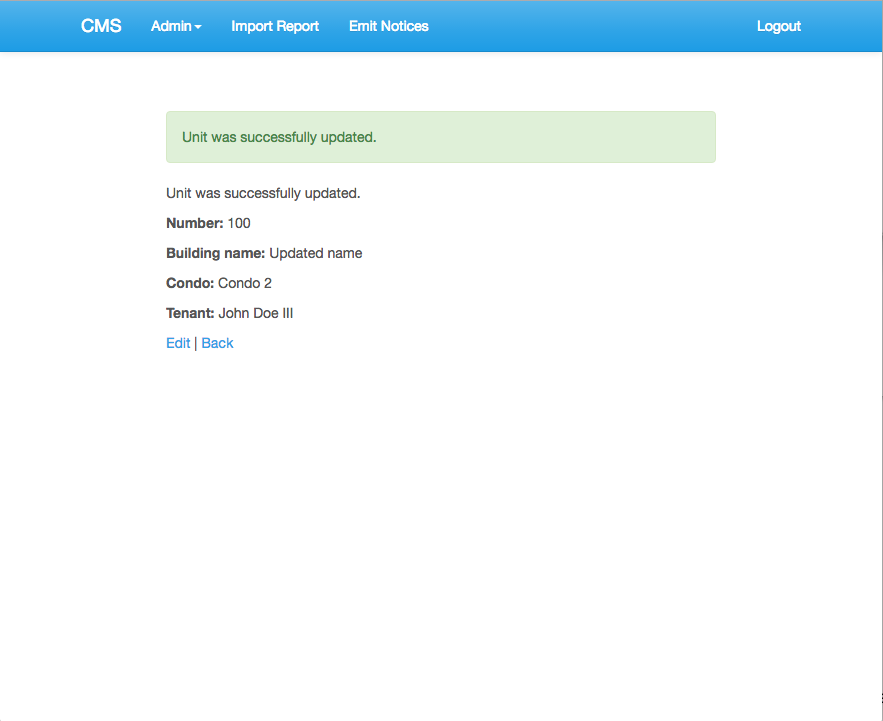
\includegraphics[scale=0.25]{./images/ss/unit/edit/5.png}
\end{itemize}

\subsection*{Delete a unit}

\begin{itemize}
  \item[] \textbf{Trigger:} User interaction with CMS window
  \item[] \textbf{Precondition:} Assert that user is in the Unit page and the unit to edit is existed
  \item[] \textbf{Path:}
    \begin{enumerate}
      \item User clicks on Destroy at the end of the information of the unit who will be deleted
      \item An alter message says ``Are you sure'' is shown
      \item User clicks ``OK'' button
      \item Unit successfully destroyed massage is shown
    \end{enumerate}
  \item[] \textbf{Requirements:}
    \begin{enumerate}
      \item The deleted unit’s data should be removed to the database
      \item The deleted unit’s information should not be displayed in the homepage
      \item Other units’ information should be listed as the same as those before deleting
    \end{enumerate}
  \item[] \textbf{Screenshots:}\\
    \includegraphics[scale=0.25]{./images/ss/unit/delete/1.png}
    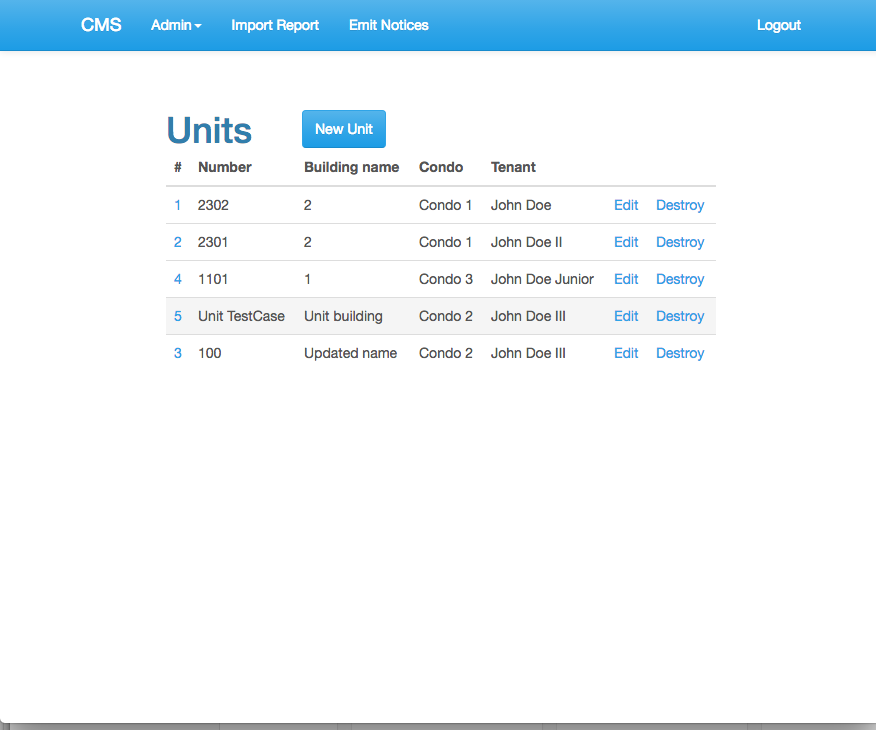
\includegraphics[scale=0.25]{./images/ss/unit/delete/2.png}\\
    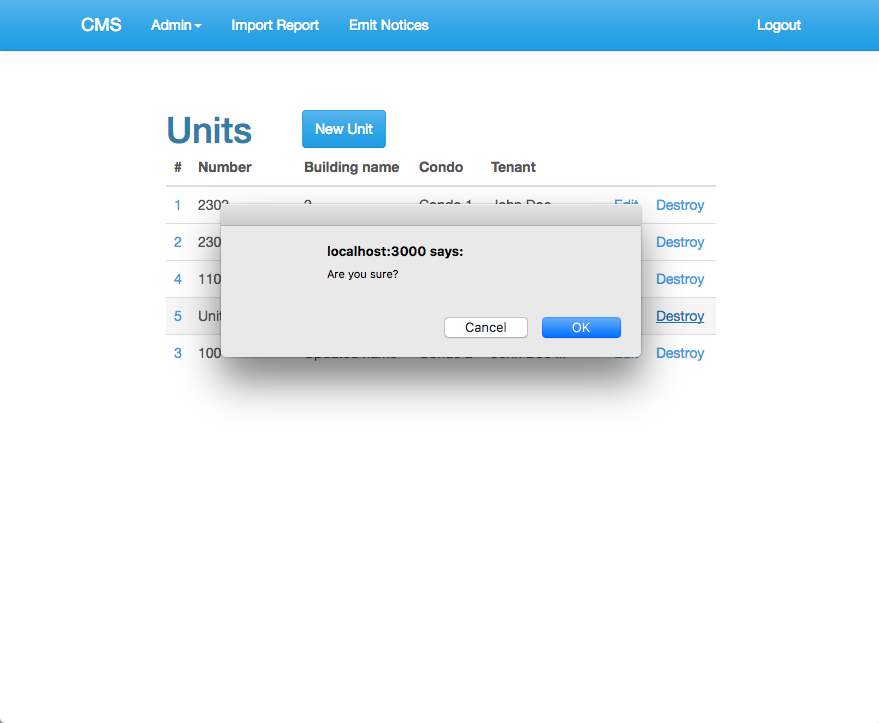
\includegraphics[scale=0.25]{./images/ss/unit/delete/3.png}
    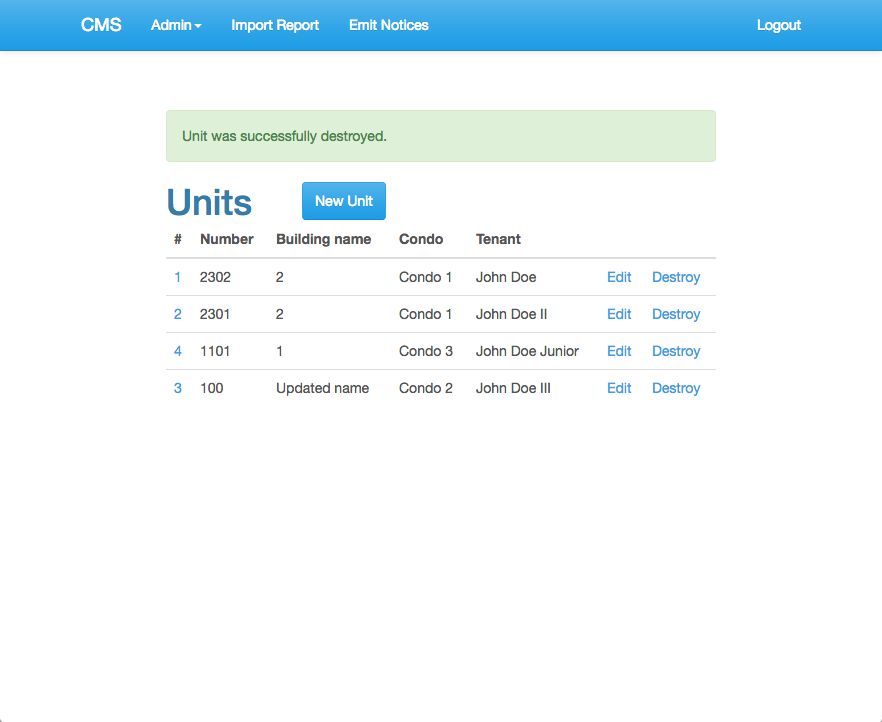
\includegraphics[scale=0.25]{./images/ss/unit/delete/4.png}
\end{itemize}
